\chapter{Nanopore Signal Analysis}
\label{cha:signal}

\begin{itemize}
	\item basic framework for development set with pipeline
	\item need to understand signal, contrast to 2nd gen.
	\item tombo, squiggle-kit? available, but not customizable regarding normalization, parameter etc.
	\item need for custom, easy to configure, python for fast prototyping
	\item fast5 format, hdfviewer, BulkVis as basic tools to work with fast5 files
\end{itemize}

\section{Simulation}
\label{sec:signal:simulation}

\begin{itemize}
    \item basic pore model
    \item base mod pore model
    \item trace with constant, time warping and noise
    \item more sophisticated simulation with simulatION, deepSimulator, scrappie, etc.
\end{itemize}


\section{Normalization}
\label{sec:signal:normalization}

\begin{itemize}
	\item mean/std vs median/MAD (cite tombo)
	\item min-max normalization with repeat signals in mind
	\item smoothing with grayscale morphological operations
	\item histogram equalization to deal with bimodal distribution of raw signal
\end{itemize}

\section{Alignment and Segmentation}
\label{sec:signal:alignment}

\begin{equation}
    s_{i,j} = max \left\lbrace \frac{c - \left| x_{i} - y_{j} \right| }{-c} \right.
\end{equation}




\begin{itemize}
	\item raw signal alignment with seqan based scoring and semi-global dp
	\item segmentation with basic image processing tools, edge filter + threshold
	\item event alignment with edlib to be more robust against time-warping
	\item profile HMM for most precise mapping
\end{itemize}

\cite{Schreiber2015}

\begin{figure}[h]
	\centering
	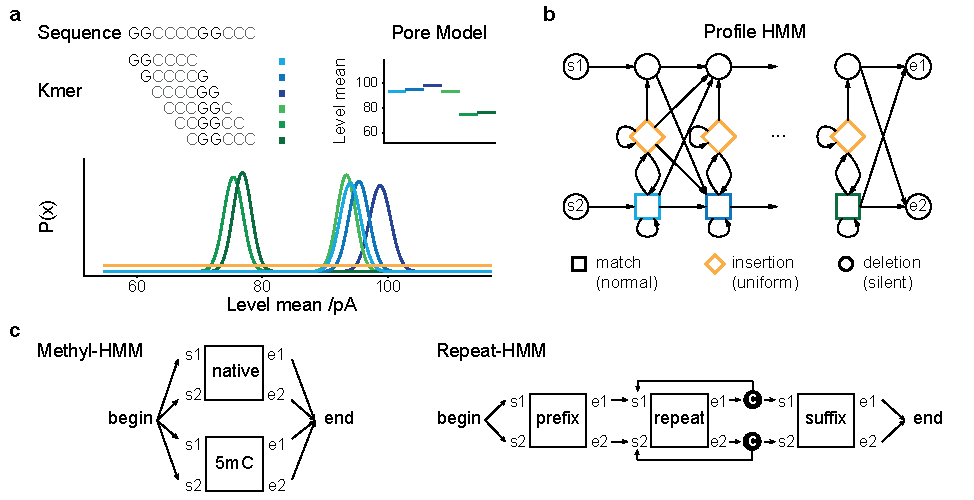
\includegraphics[width=1.0\textwidth]{figures/signal/count_hmm.pdf}
	\captionsetup{format=plain}
	\caption[Nanopore signal processing with STRique]{\textbf{a}, A compound profile HMM of prefix, a single repeat and the suffix sequence assigns either prefix, repeat or suffix label to each signal value. Repeat counts are obtained through dummy states between repeat and suffix. \textbf{b}, Nanopore signal profile HMM with normal distributed match state and uniform distributed insertion state emission probabilities.}
	\label{fig:strique:count_hmm}
\end{figure}